%!TEX program = xelatex
%!LW recipe=latexmk (xelatex)
% LTeX: enabled=true

\documentclass{article}

\input{style.sty}

\title{\bfseries Dome Inspection and Metrology}
\author{Alan M.\ Watson}
\date{10 March 2026}

\usepackage{graphicx}

\begin{document}
\maketitle

\section{Context}

In the first week of December 2025, the neoprene seal between the building and the dome was damaged. It appears to have been torn at the point that it is fixed by steel strips to the interface plates attached to the building. It fell between the dome and building on the SW side and prevented movement. On-site staff removed the damaged seal between azimuths of about 150 and 330 degrees and fixed the ends of the undamaged seal so that the dome could turn. See Figure~\ref{figure:damaged-seal}.

Unsurprisingly, water is now able to penetrate the enclosure and reach the interface plate. See Figure~\ref{figure:water}.

\begin{figure}
    \centering
    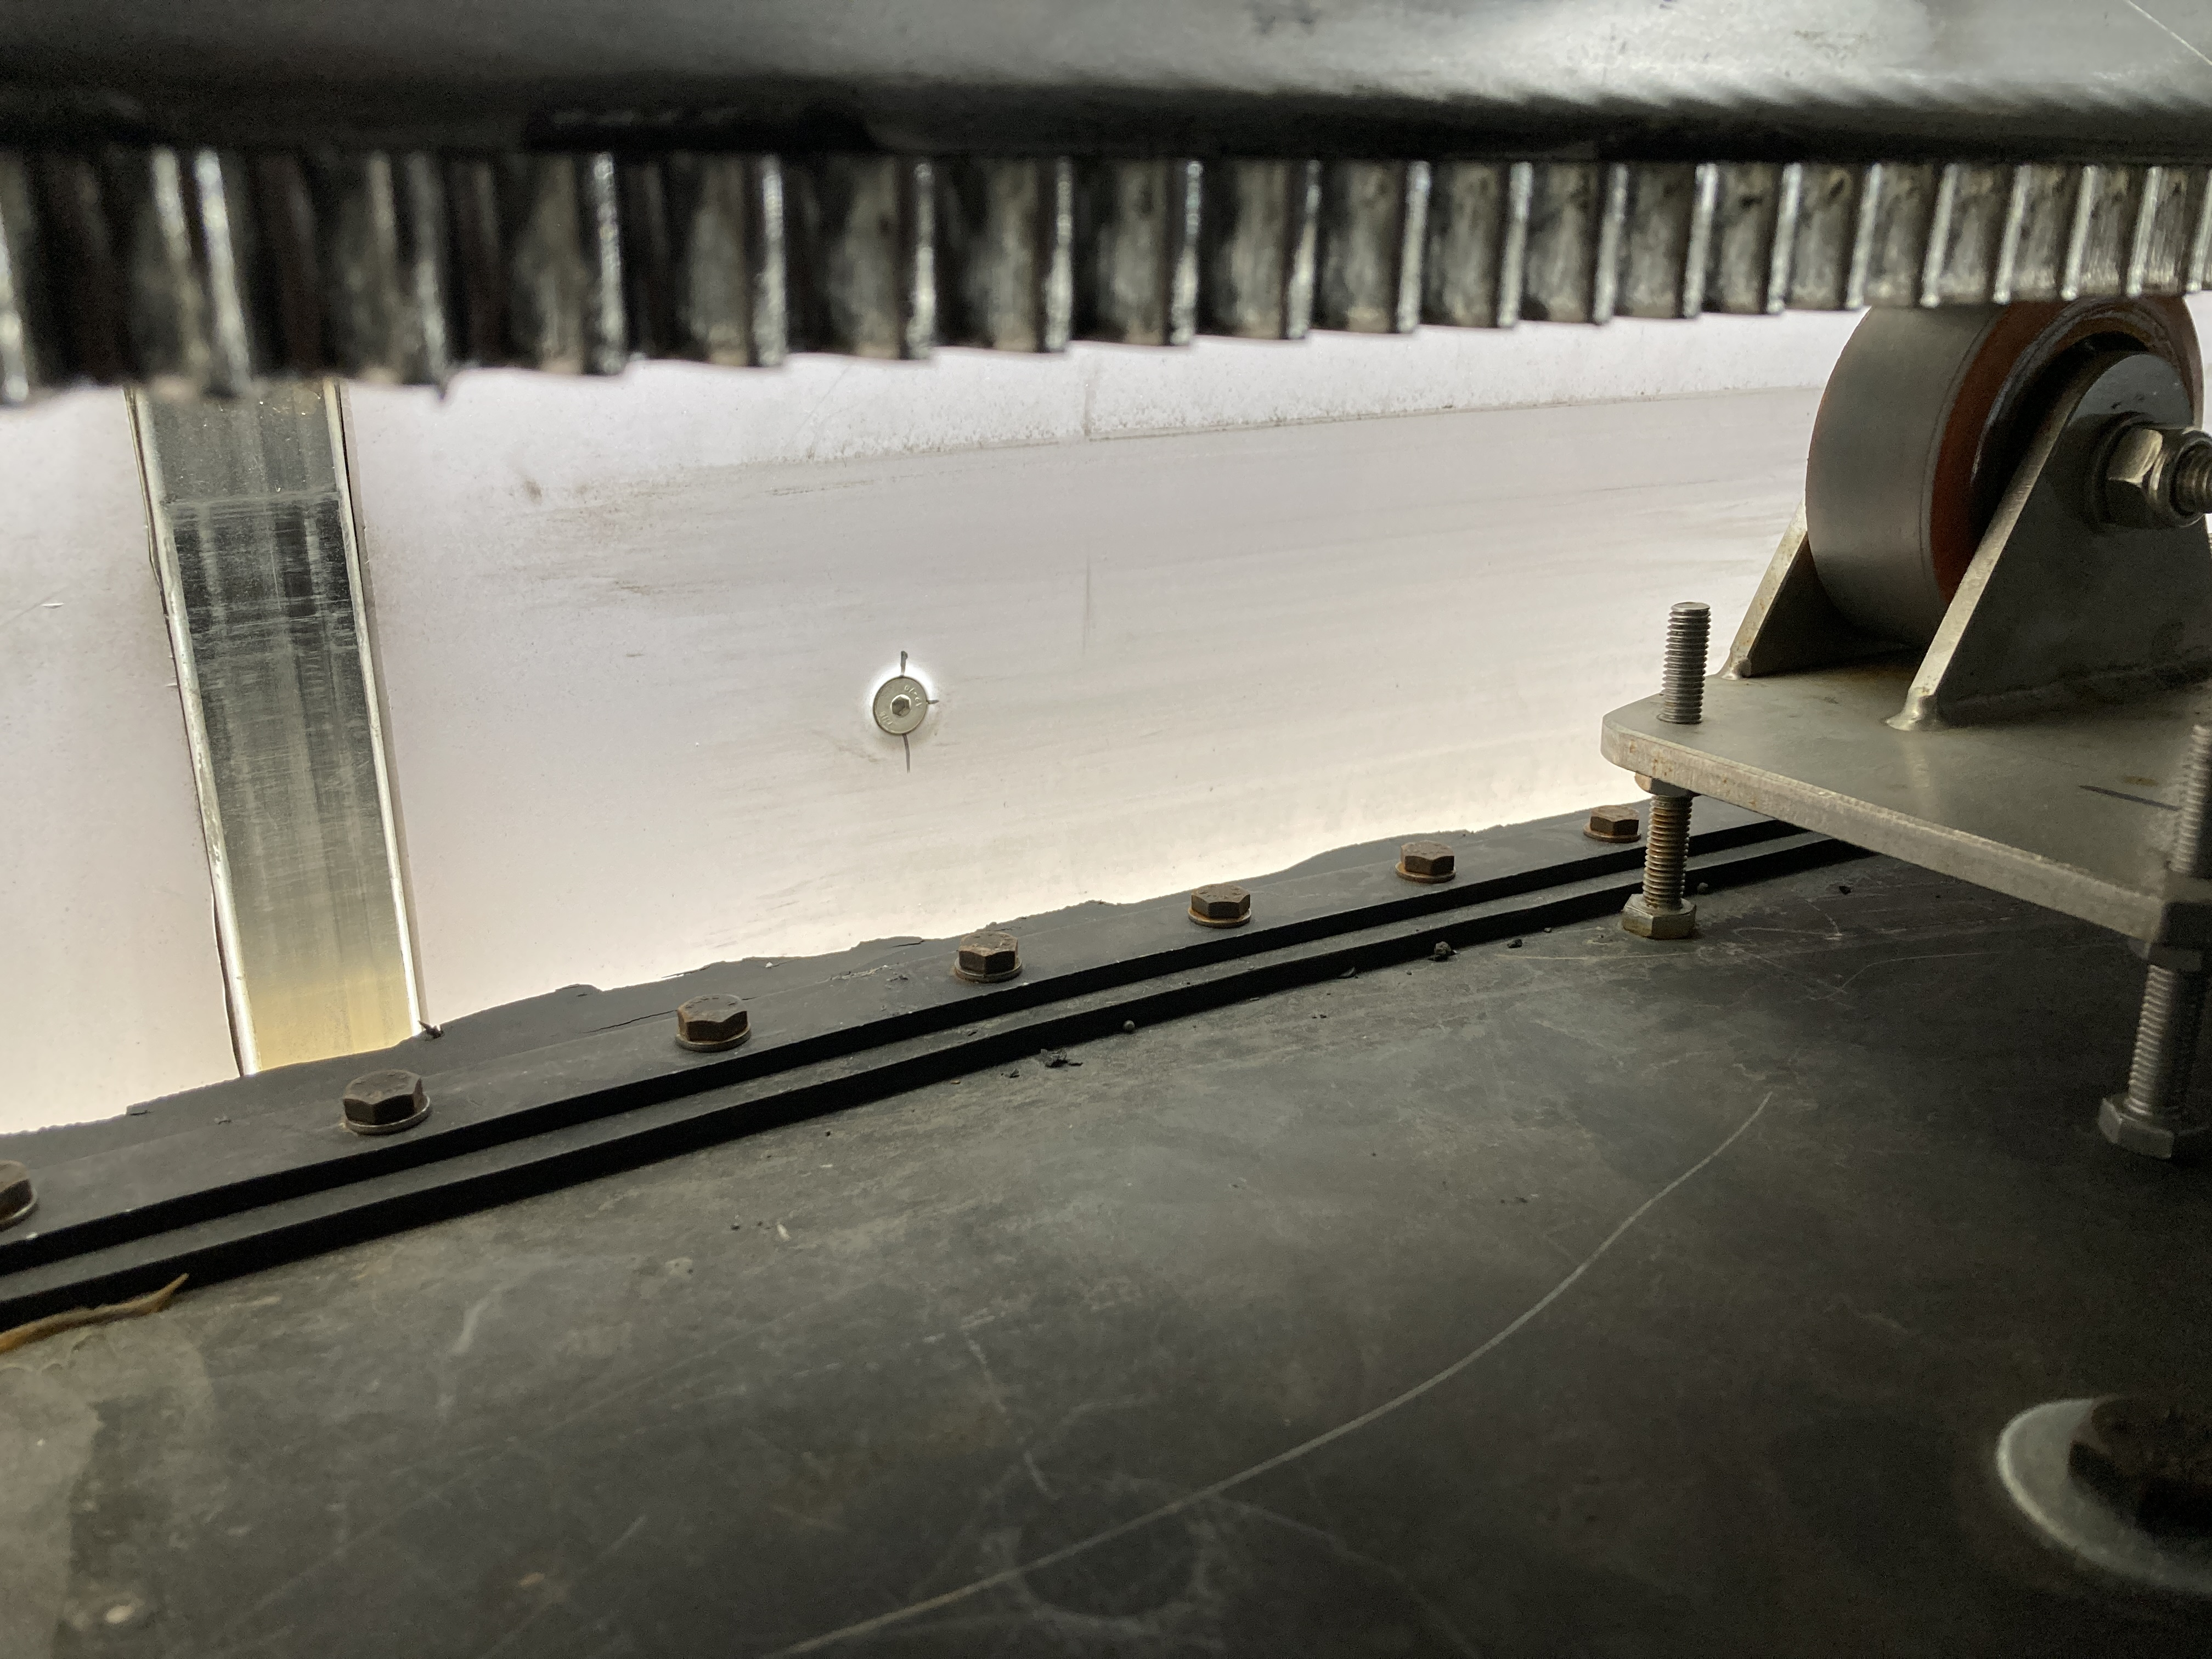
\includegraphics[width=0.8\linewidth]{IMG_6041.JPG}
    \caption{The damaged seal.}
    \label{figure:damaged-seal}
\end{figure}

\begin{figure}
    \centering
    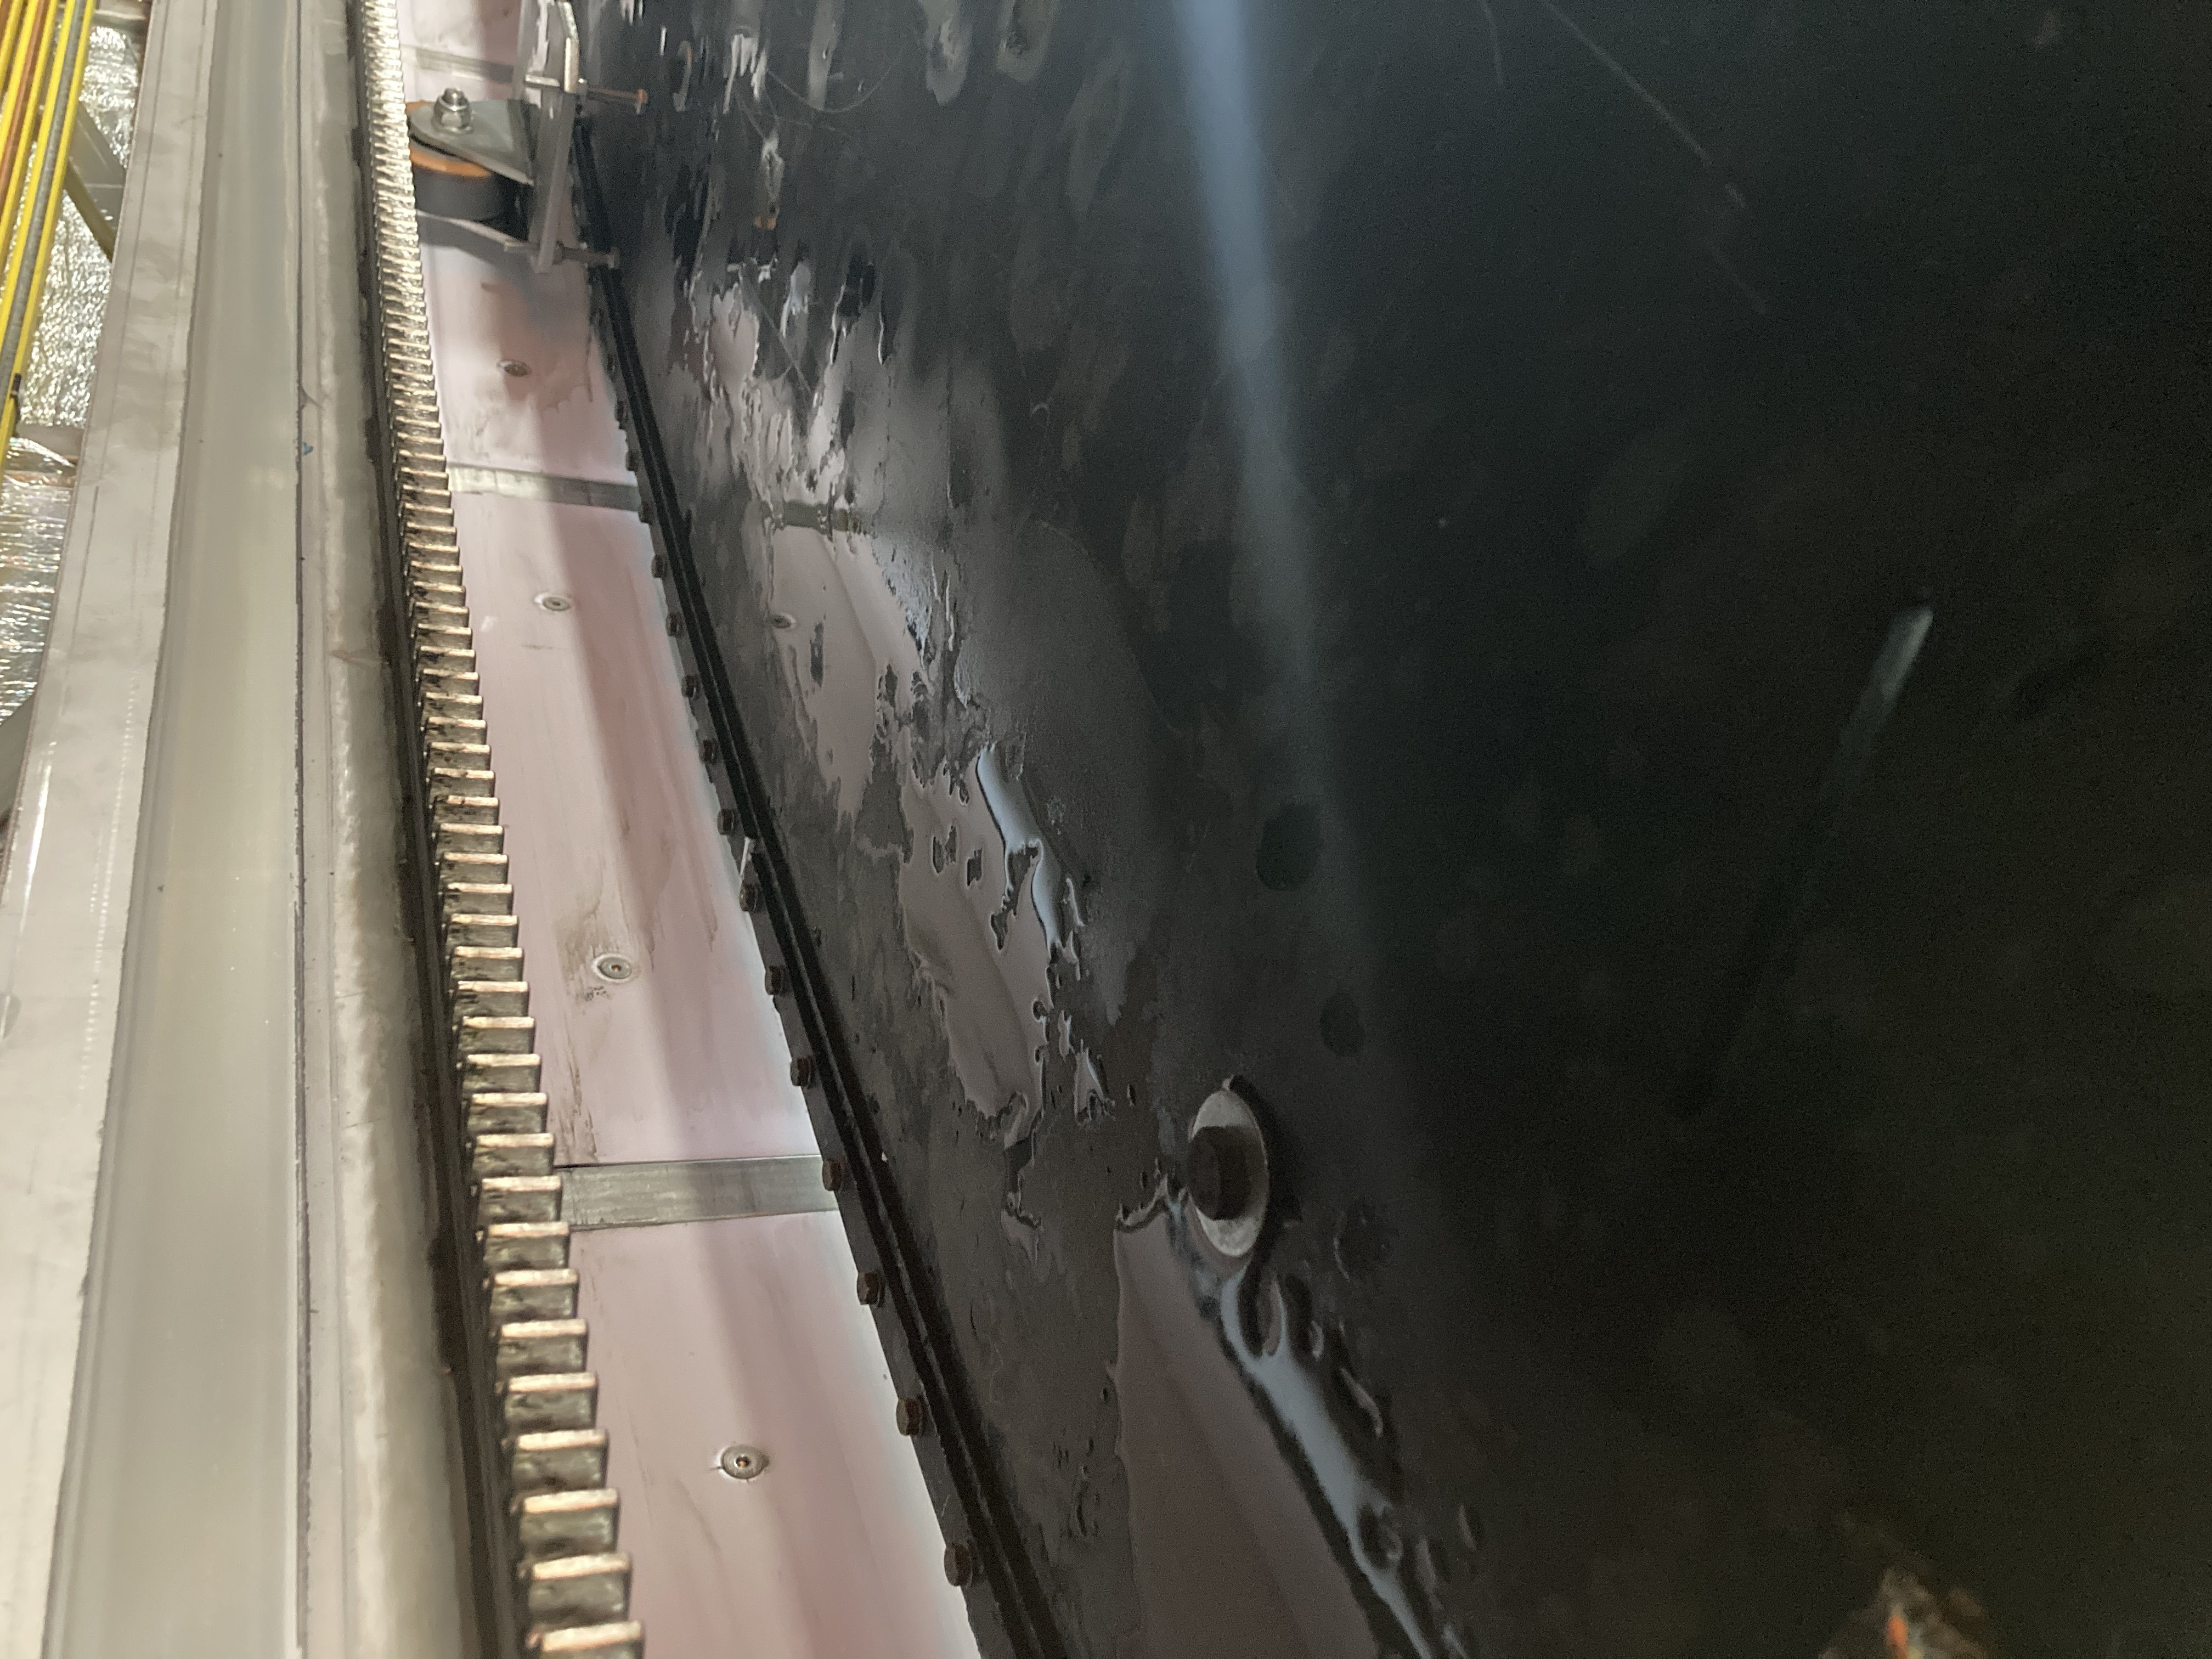
\includegraphics[height=0.6\linewidth,angle=-90]{IMG_6085.JPG}
    \caption{Water on the interface plate.}
    \label{figure:water}
\end{figure}

\section{Are the Supports Damaged or Displaced?}

During December 2025, I inspected the radial and vertical supports of the dome. I found no evidence that any of them were damaged, bent, or had moved.

\section{Is the Dome Centered?}

\subsection{Metrology}

During December 2025, with the help of Santiago Paez, I performed metrology on the dome.

All azimuths are measured from north through east. We assume the northernmost radial support is at an azimuth of zero. This support is not precisely aligned with true geographical north, but it is close, and this support provides a convenient reference.

\begin{figure}
    \centering
    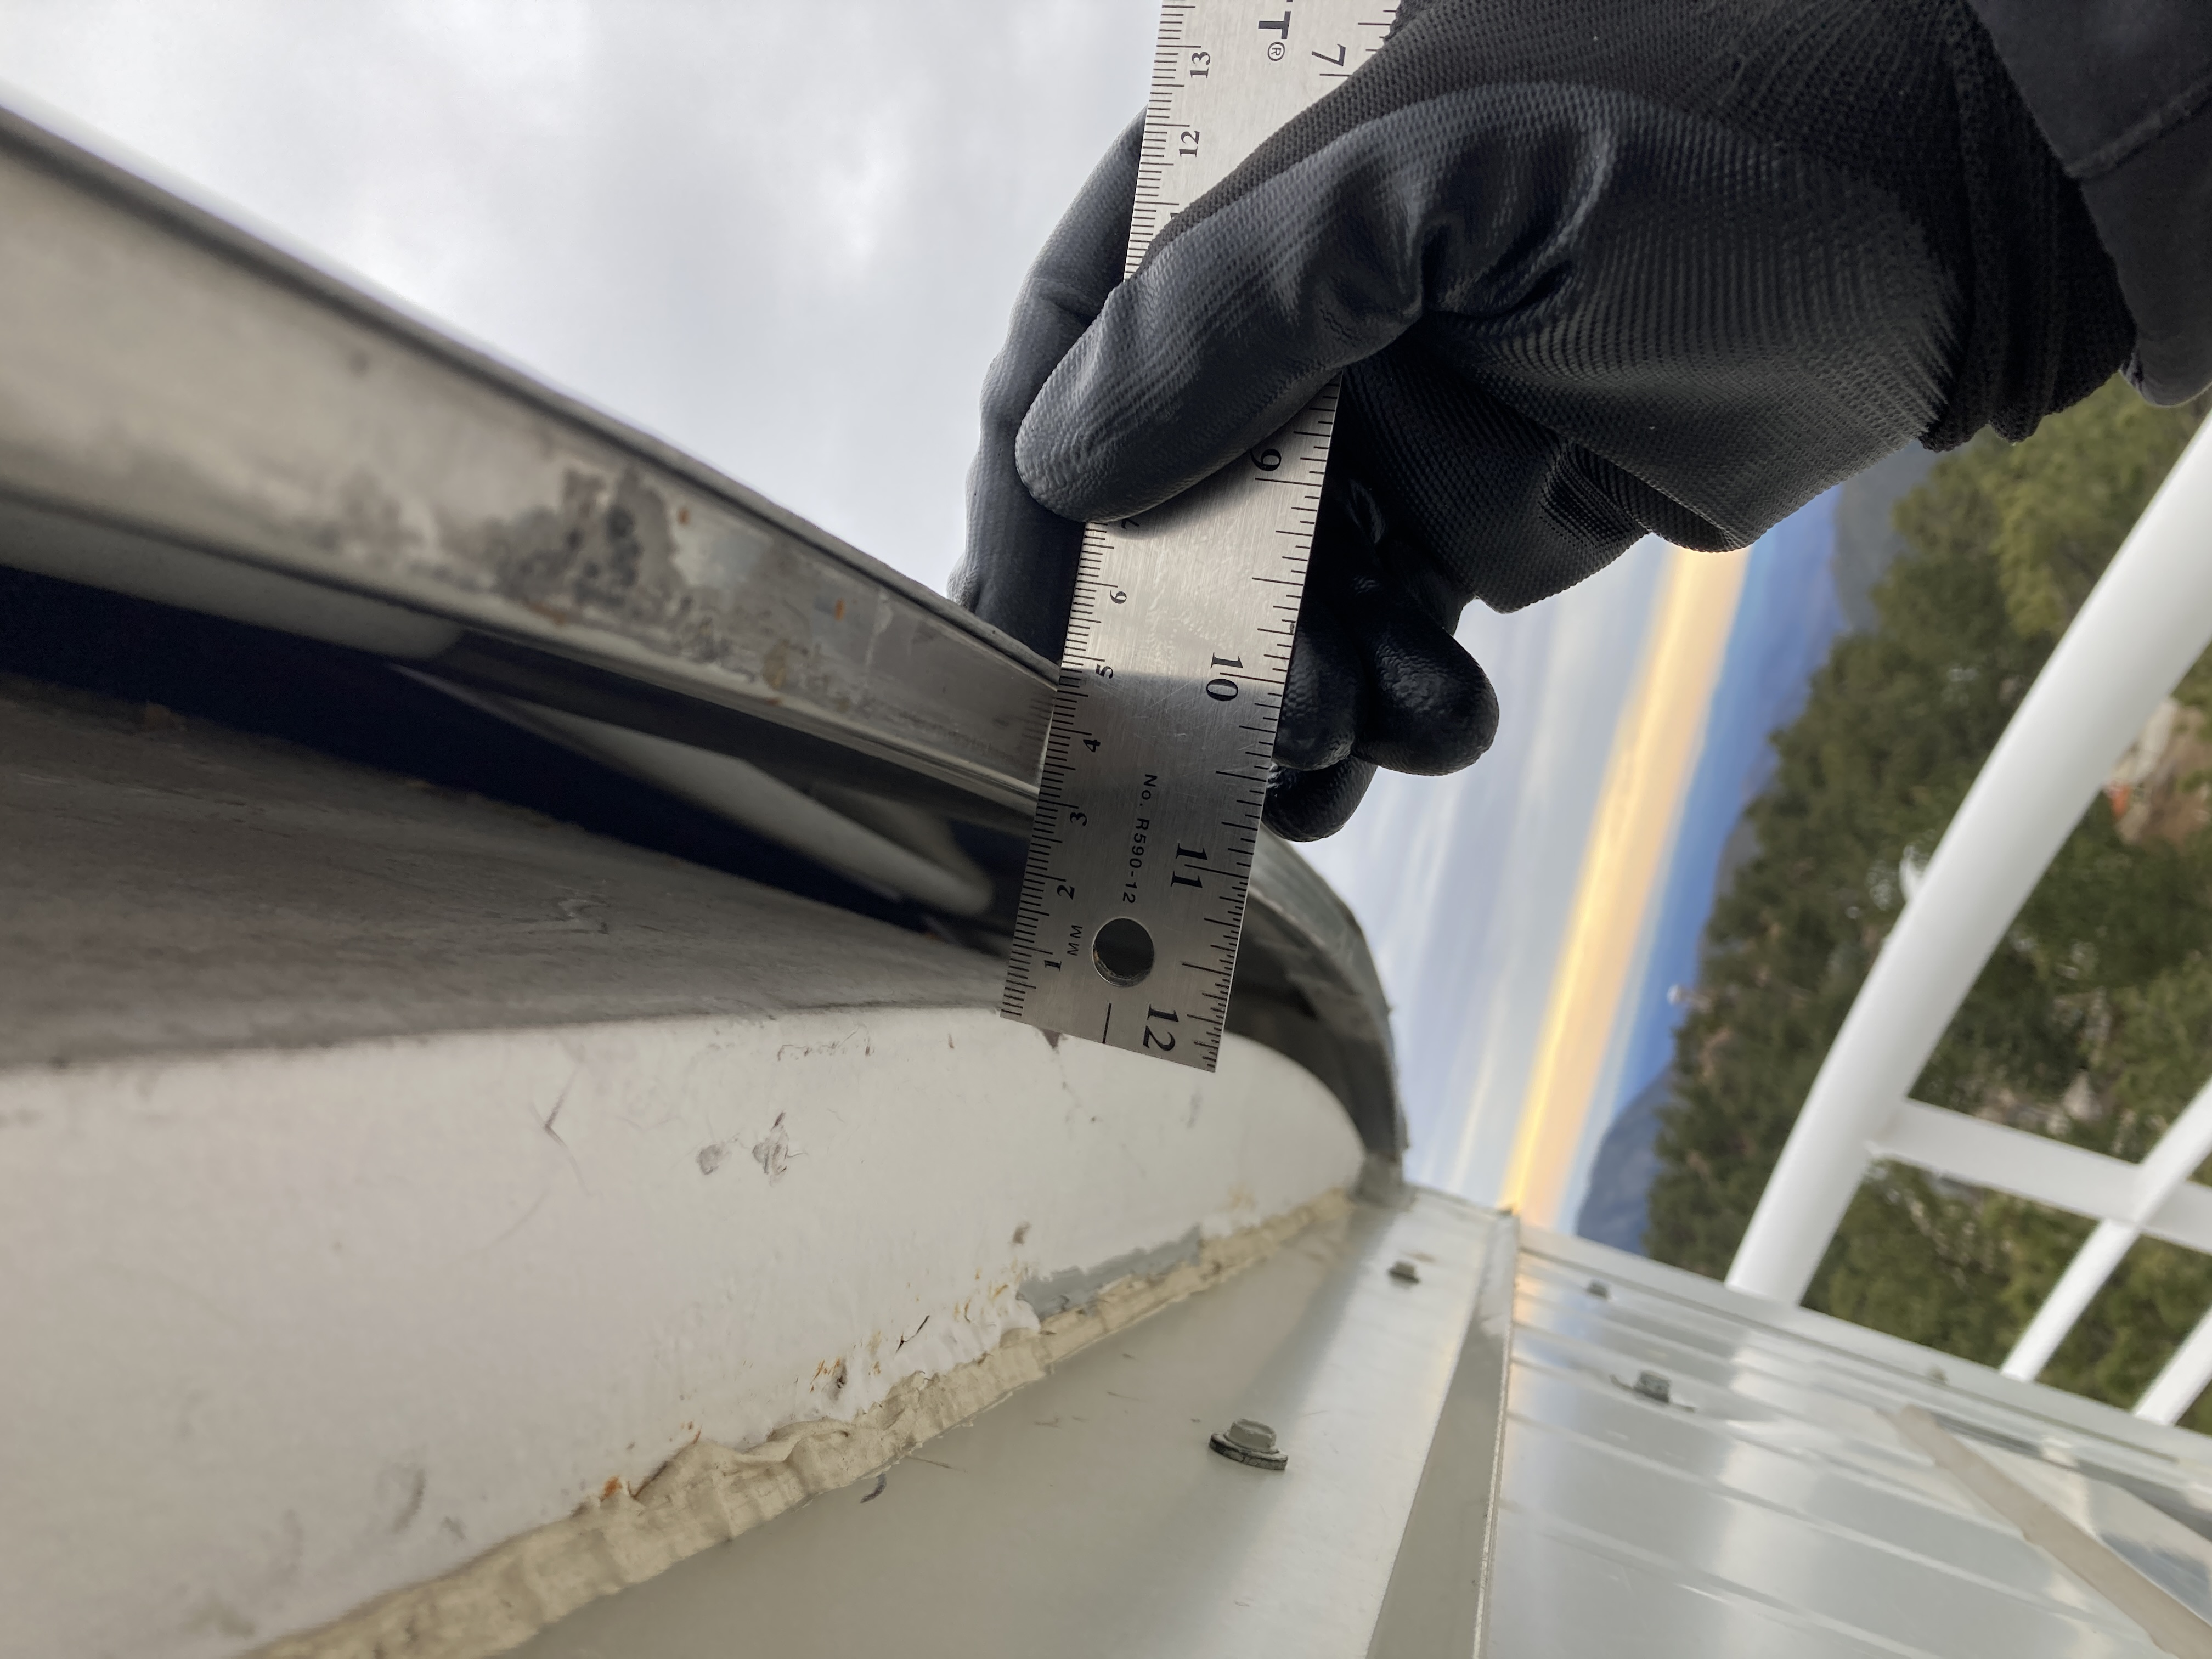
\includegraphics[height=0.4\linewidth,angle=-90]{IMG_6077.JPG}
    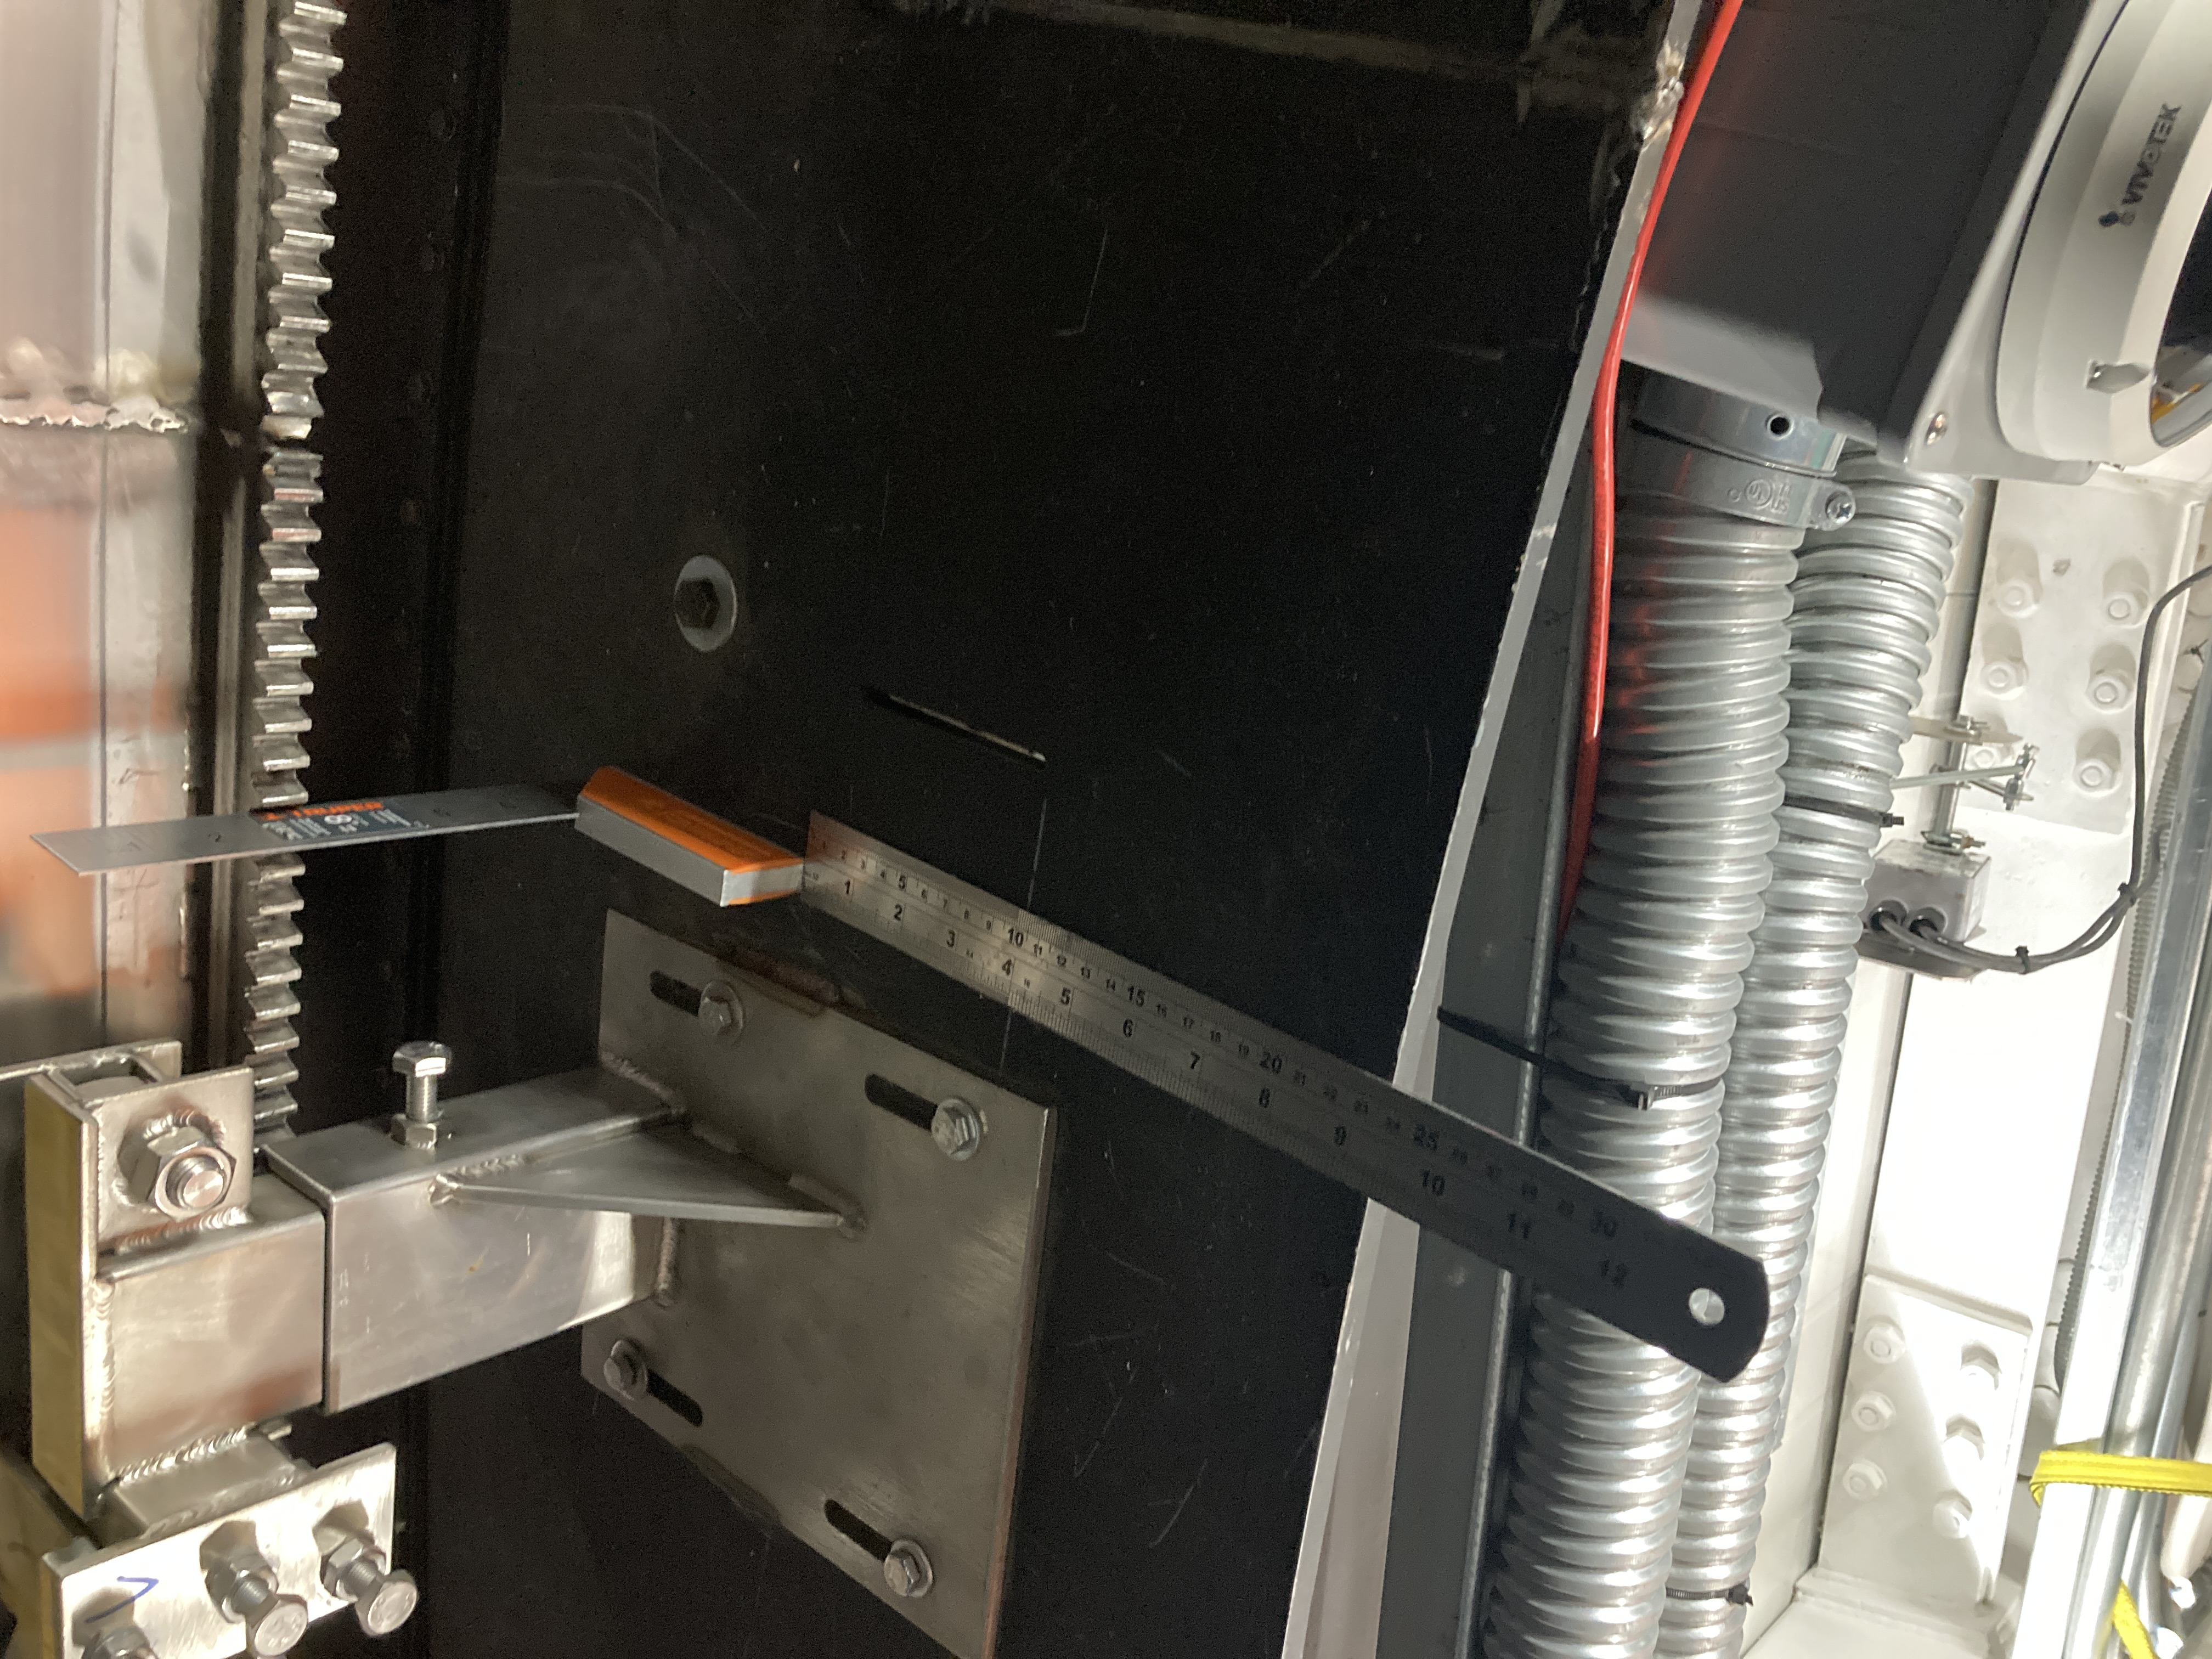
\includegraphics[height=0.4\linewidth,angle=-90]{IMG_6084.JPG}

    \caption{Left: Measuring the distance $D$ between the outer radius of the building beam and inner radius of the dome.
    Right: Measuring the distance $G$ from the inner radius of the interface plates to the bottom of the teeth in the drive track.}
    \label{figure:measurement-D-and-G}
\end{figure}

\begin{figure}
    \centering

    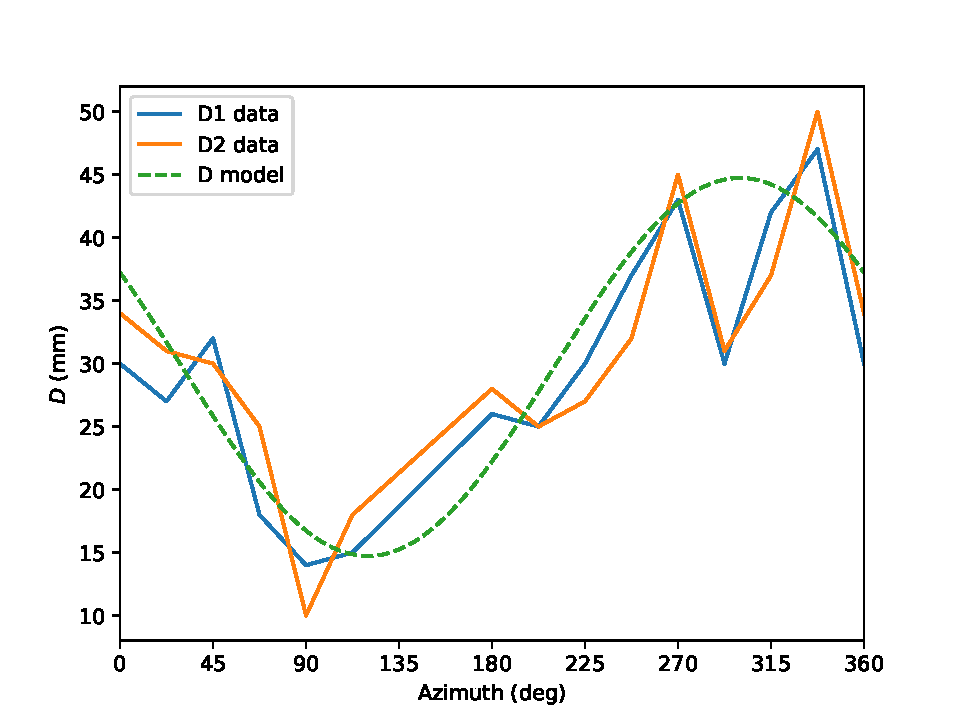
\includegraphics[width=0.8\linewidth]{plot-D.pdf}
    \caption{The distance $D$ between the outer radius of the building beam and inner radius of the dome as a function of azimuth. The plot shows two sets of measurements ($D1$ and $D2$) and an approximate sinusoidal model with a half-amplitude of 15 mm and a maximum at 300 deg.}
    \label{figure:plot-D}

    \vspace{\floatsep}

    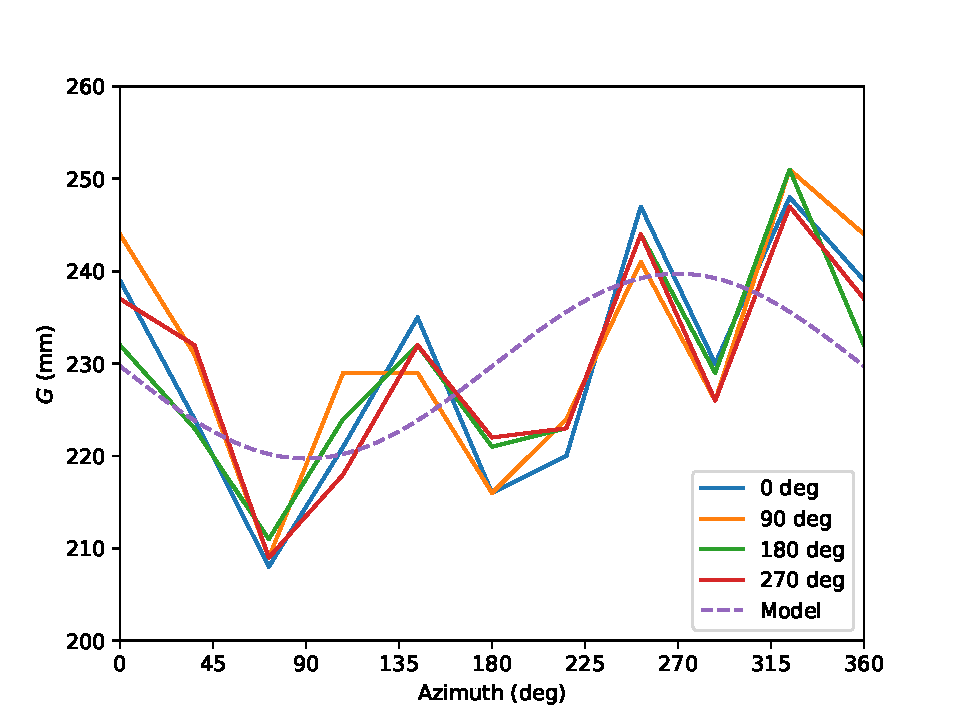
\includegraphics[width=0.8\linewidth]{plot-G.pdf}
    \caption{The distance $G$ between from the inner radius of the interface plates to the bottom of the teeth in the drive track as a function of azimuth and for the dome shutter at azimuths of 0, 90, 180, and 270 deg. The plot also shows approximate sinusoidal model with a half-amplitude of 11 mm and a maximum of 285 deg.}
    \label{figure:plot-G}

\end{figure}

\begin{table}
    \centering

    \caption{Values of $D1$ and $D2$}
    \label{table:D}
    \medskip
    \begin{tabular}{rrr}
        \toprule
        $A$&$D1$&$D2$\\
        (deg)&(mm)&(mm)\\
        \midrule
        0.0&30&34\\
        22.5&27&31\\
        45.0&32&30\\
        67.5&18&25\\
        90.0&14&10\\
        112.5&15&18\\
        180.0&26&28\\
        202.5&25&25\\
        225.0&30&27\\
        247.5&37&32\\
        270.0&43&45\\
        292.5&30&31\\
        315.0&42&37\\
        337.5&47&50\\
        \bottomrule
    \end{tabular}

    \vspace{\floatsep}

    \caption{Values of $G$}
    \label{table:G}
    \medskip
    \begin{tabular}{rrrrr}
        \toprule
        $A$&$G0$&$G90$&$G180$&$G270$\\
        (deg)&(mm)&(mm)&(mm)&(mm)\\
        \midrule
        0.0&236&241&229&234\\
        36.0&228&235&227&236\\
        72.0&216&217&219&217\\
        108.0&231&239&234&228\\
        144.0&243&237&240&240\\
        180.0&219&219&224&225\\
        216.0&216&220&219&219\\
        252.0&239&233&236&236\\
        288.0&220&216&219&216\\
        324.0&240&243&243&239\\
        \bottomrule
    \end{tabular}
\end{table}

\begin{figure}
    \centering

    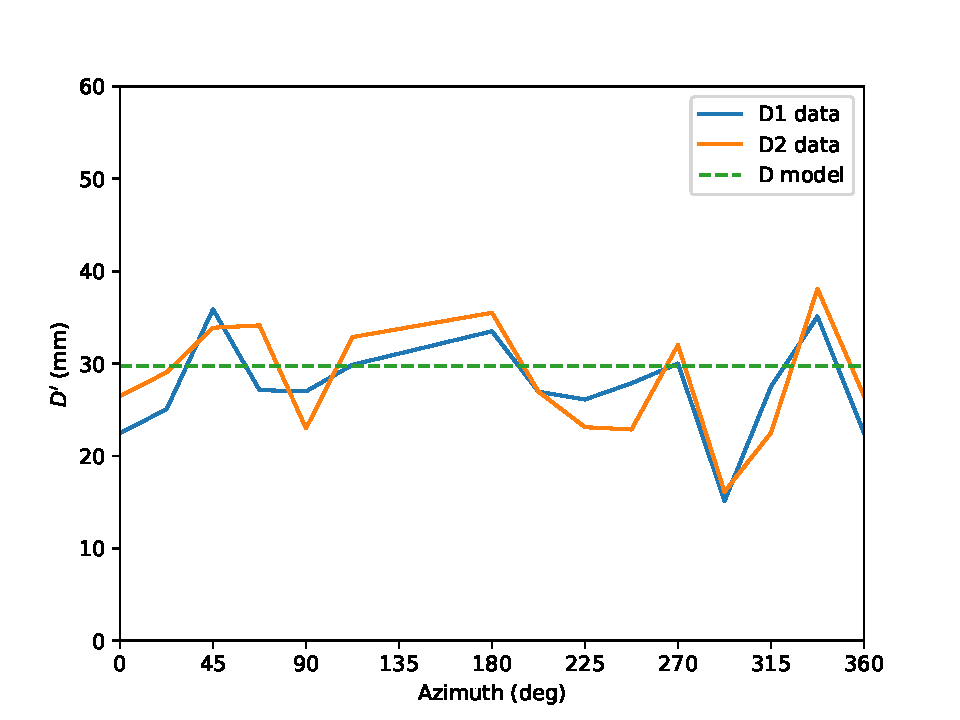
\includegraphics[width=0.8\linewidth]{plot-D-prime.pdf}
    \caption{The estimated distance $D'$ between the outer radius of the building beam and inner radius of the dome as a function of azimuth after displacing the dome by 15 mm at an azimuth of 120 degrees. The model assumes the dome moves rigidly.}
    \label{figure:plot-D-prime}

    \vspace{\floatsep}

    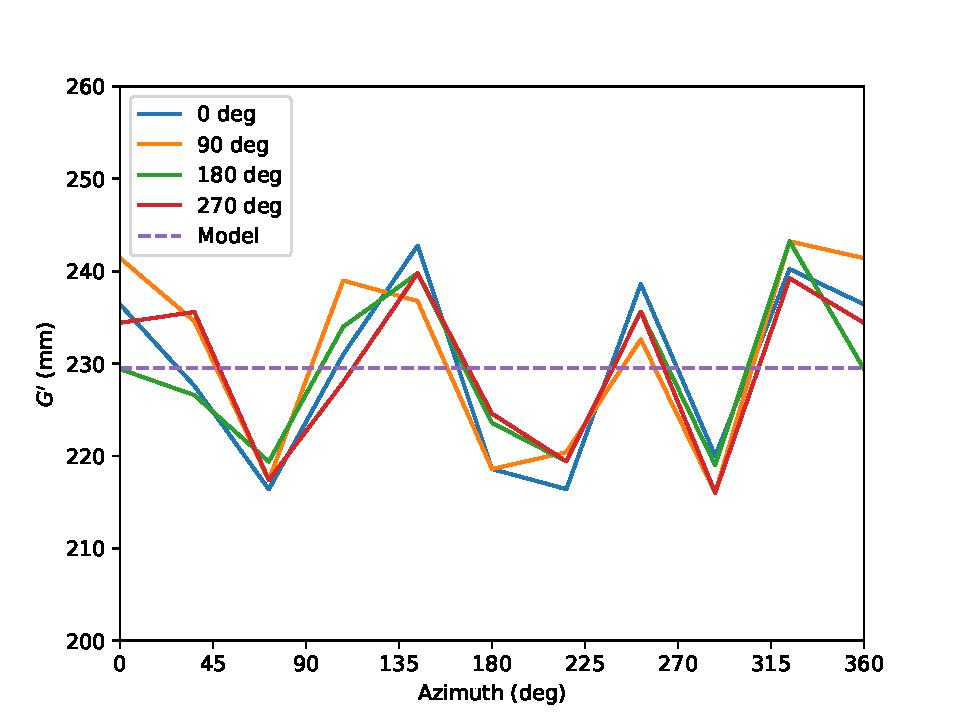
\includegraphics[width=0.8\linewidth]{plot-G-prime.pdf}
    \caption{The estimated distance $G'$ between from the inner radius of the interface plates to the bottom of the teeth in the drive track as a function of azimuth and for the dome shutter at azimuths of 0, 90, 180, and 270 deg after displacing the dome by 11 mm at an azimuth of 105 degrees. The model assumes the dome moves rigidly.}
    \label{figure:plot-G-prime}
\end{figure}

We measured the distance $D$ between the outer radius of the beam on the building and the inner radius of the dome at the center of 14 of the 16 sides of the building. See Figure~\ref{figure:measurement-D-and-G}. We were not able to measure this at two positions over the door. The dome was positioned with the slit to the north. We repeated the measurement twice ($D1$ and $D2$) to confirm that the apparently anomalous point at 292.5 degrees is correct.

We also measured the distance $G$ from the inner radius of the interface plates to the bottom of the teeth in the drive track. See Figure~\ref{figure:measurement-D-and-G}. (More precisely, we measured this distance minus the length of one side of the set-square, but since we are interested only in differences this is irrelevant.) We obtained measurements with the dome shutter at azimuths of 0, 90, 180, and 270 degrees. We measured this at each one of the 10 radial supports.

The results are shown in Figures~\ref{figure:plot-D} and \ref{figure:plot-G} along with sinusoidal models (fit by eye). The raw data are shown in Tables~\ref{table:D} and \ref{table:G}. 

Figure~\ref{figure:plot-D} suggests that the dome is displaced with respect to the building by about 15~mm, being furthest from the building at an azimuth of about 300 degrees (WNW) and closest at about 120 degrees (ESE). At its widest point, the gap is almost 50 mm, but at its narrowest point it is about 15 mm. Figure~\ref{figure:plot-G} suggests that the dome is displaced with respect to the interface plate by about 11~mm, being furthest from the building at an azimuth of about 285 degrees (between W and WNW) and closest at about 105 degrees (between E and ESE). These two estimated displacements are similar but not identical; it is possible that the interface plate is not perfectly centered on the building. Nevertheless, we can conclude that the dome is displaced by 10--15 mm towards W or WNW with respect to both the building and the interface plate.


\subsection{Nominal Recentering}

Figure~\ref{figure:plot-D-prime} shows $D'$, the value of $D$ after displacing the dome by 15~mm at an azimuth of 120 degrees, assuming the dome moves rigidly. The P-V is reduced from 40 mm to 23 mm. Figure~\ref{figure:plot-G-prime} shows $G'$, the value of G after displacing the dome by 11~mm at an azimuth of 105 degrees, assuming the dome moves rigidly. The P-V is reduced from 43 to 27 mm.

\subsection{Variations after Nominal Recentering}

Even after modeling the displacement of the dome to better center it, there are still notable variations in $D'$ and $G'$. For example, in Figure~\ref{figure:plot-D-prime} the measurement at 292.5 deg is approximately 15 mm smaller than the general trend (i.e., the dome is 15 mm closer to the building than the general trend). A similar deviation is seen in Figure~\ref{figure:plot-G-prime}, in which the measurement at 288 deg is approximately 10 mm smaller than the general trend. The similarity between these and other residuals suggests that they are real. 

One possibility is that these residuals reflect variations in the radial position of the radial supports; that is that the radial supports are forcing the dome outwards at some positions (the high residuals, e.g., at about 135 and 340 degrees) and allowing it to move inwards at other positions (the low residuals, e.g., at about 280 degrees). If this is the case, the dome may be undergoing repeated deformations, which could damage it and the radial supports and cause additional load on the motors.

\subsection{Conclusions}

\begin{itemize}
    \item The dome appears to be decentered with respect to both the building (measurement $D$) and the interface plate (measurement $G$). The displacements are estimated to be 15 and 11 mm, respectively, at azimuths of 300 and 285 degrees. These are in fairly good agreement.
    \item After subtracting a model that corresponds to a nominal recentering of the dome, there are still significant residuals in the radial measurements $D'$ and $G'$. These may be caused by local deformations of the dome by the radial supports.
\end{itemize}

\section{Discussion}

There is no evidence that any of the supports are damaged or have moved.

The dome is currently decentered. We would assert that the dome has not moved, but was installed decentered. The original seal, which was installed between the building and the dome, tore in the east, precisely where the clearance between the dome and the building was and is smallest. When ASTELCO came a second time in the summer of 2024 to install the telescope and work on the dome, it was clear that the dome was closest to the building in the east; this is where we had to be most careful of the clearance when expanding the dome at its lower edge. The gap between the building and dome to the west has \emph{always} been wider than the gap to the east.

It seems the first thing to do is to correct this consequence of the installation and recenter the dome. As part of this process, we might also consider if the radial supports are locally deforming the dome out of a circular shape and, if necessary and possible, correct this.

\end{document}